\documentclass[11pt,oneside,a4paper,final]{article}

\usepackage{fancyhdr}
\usepackage{lastpage}

\pagestyle{fancy}

\renewcommand{\headrulewidth}{0.0pt}

\lhead{}
\chead{}
\rhead{}
\lfoot{}
\cfoot{Page {\thepage} of \pageref{LastPage}}
\rfoot{}

\usepackage{longtable}

\usepackage[style=numeric,backend=biber]{biblatex}
% \usepackage[style=numeric]{biblatex}
\bibliography{install}
\usepackage{hyperref}
\usepackage[paper=a4paper,margin=1.6cm]{geometry}	% 1 inch margins all around
\usepackage[british=nohyphenation]{hyphsubst}
\usepackage[british]{babel}
\usepackage{graphicx}
\usepackage[caption=false,font=normalsize,labelfont=sf,textfont=sf]{subfig}
\usepackage[acronym,toc]{glossaries}
\makeglossaries
% \phantomsection
% \addcontentsline{toc}{section}{Acronyms}
% \section*{Acronyms}
% \begin{footnotesize}
% \begin{acronym}[TDMA]

% \newacronym{2D}{2D}{two-dimensional}
\newacronym{3D}{3D}{three-dimensional}
\newacronym{FBO}{FBO}{frame buffer object}
\newacronym{FLTK}{FLTK}{Fast Light Toolkit}
\newacronym{GLEW}{GLEW}{OpenGL Extension Wrangler Library}
\newacronym{GLSL}{GLSL}{OpenGL Shading Language}
\newacronym{GLU}{GLU}{OpenGL Utility Library}
\newacronym{GLUT}{GLUT}{OpenGL Utility Toolkit}
\newacronym{GPU}{GPU}{Graphics Processor Unit}
% \newacronym{GUI}{GUI}{graphical user interface}
% \newacronym{Gzip}{Gzip}{GNU zip}
% \newacronym{ITK}{ITK}{Insight Segmentation and Registration Toolkit}
\newacronym{keV}{keV}{kiloelectron volt}
% \newacronym{MXE}{MXE}{M cross environment}
\newacronym{STL}{STL}{STereoLithography}
\newacronym{SVN}{SVN}{Subversion}
\newacronym{VBO}{VBO}{vertex buffer object}
% \newacronym{VTK}{VTK}{Visualization Toolkit}
% 


\title{gVirtualXRay -- Installation Guide}
\author{Dr Franck P. Vidal}
\date{31\textsuperscript{th} August 2016}

\begin{document}
 \sloppy

\maketitle

\newpage
\phantomsection
\addcontentsline{toc}{section}{Table of contents}
\tableofcontents

% \newpage
% \phantomsection
% \addcontentsline{toc}{section}{List of figures}
% \listoffigures
% 
\newpage
\phantomsection
\addcontentsline{toc}{section}{List of tables}
\listoftables

\newpage


\section{Requirements}

	We rely on the \href{http://www.cmake.org/}{CMake} toolchain. 
	To make life easy, we have decided to automatically download and compile most of the software libraries in the build tree. 
	It is optional, of course, in case you want to use your system's libraries. 
	The default behaviour is to let CMake download and install the dependencies.
	The list of tools and libraries required to build gVirtualXRay is summarised in Table~\ref{tab:requiredToolsAndLibraries}.

\begin{table}[tbhp]
	\begin{center}
		\caption{\label{tab:requiredToolsAndLibraries} Tools and libraries required to build gVirtualXRay. Components marked with (*) cannot be installed automatically.} 
		\begin{small}
			\begin{tabular}{|c|c|c|c|p{0.3\linewidth}|}
				\hline
				\textbf{Name} &\textbf{Component} & \textbf{Platform} & \textbf{Status} & \textbf{URL}\\
				\hline
				\hline
				C++ compiler  & Development tool & Linux, Mac OS X \& Windows & Required & Platform dependant\\
				\hline
				CMake (*)  & Development tool & Linux, Mac OS X \& Windows & Required & \url{http://www.cmake.org/}\\
				\hline
				OpenGL (*) & Library & Linux, Mac OS X \& Windows & Required & \url{http://www.opengl.org/}\\
				\hline
				\Acrshort{Gzip} & System tool & Linux, Mac OS X \& Windows & Required & \url{http://www.gzip.org/}\\
				\hline
				\Acrshort{GLEW} & Library & Linux, Mac OS X \& Windows & Required & \url{http://glew.sourceforge.net/}\\
				\hline
				Zlib & Library & Linux, Mac OS X \& Windows & Required & \url{http://www.zlib.net/}\\
				\hline
				FreeType & Library & Linux, Mac OS X \& Windows & Optional & \url{http://www.freetype.org/}\\
				\hline
				\Acrshort{GCDM} & Library & Linux, Mac OS X \& Windows & Optional & \url{http://gdcm.sourceforge.net/}\\
				\hline
				LibTIFF & Library & Linux, Mac OS X \& Windows & Optional & \url{http://www.libtiff.org/}\\
				\hline
				XCOM & Database & Linux, Mac OS X \& Windows & Optional & \url{http://physics.nist.gov/PhysRefData/Xcom/Text/download.html}\\
				\hline
				GLFW & Library & Linux, Mac OS X \& Windows & Optional & \url{http://www.glfw.org/}\\
				\hline
				GLUT & Library & Linux, Mac OS X \& Windows & Optional & \url{http://freeglut.sourceforge.net/}\\
				\hline
				\Acrshort{FLTK} & Library & Linux, Mac OS X \& Windows & Optional & \url{http://www.fltk.org/}\\
				\hline
				Qt4 (*) & Library & Linux, Mac OS X \& Windows & Optional & \url{https://www.qt.io/}\\
				
				Qt4 COMPONENTS QtCore QtGui QtOpenGL
				\hline
				Qt5 (*) & Library & Linux, Mac OS X \& Windows & Optional & \url{https://www.qt.io/}\\
				
				find_package(Qt5Gui)
find_package(Qt5Widgets)
find_package(Qt5OpenGL)

				
				\hline
				Doxygen (*) & Development tool & Linux, Mac OS X \& Windows & Optional & \url{http://www.doxygen.org/}\\
				\hline
			\end{tabular}
		\end{small}
	\end{center}
\end{table}

	\subsection{Linux}

To my knowledge, g++, CMake, make, gzip Qt4, Qt5 and Doxygen are official packages on every Linux system. 
The version I have tested are:

\begin{itemize}
\item Linux system: OpenSUSE Leap 42.1, x86_64
\item g++: 4.8.5
\item CMake: 3.3.2
\item make: GNU Make 4.0
\item gzip: 1.6
\item Qt4: 4.8.6
\item Qt5: 5.5.1
\item Doxygen: 1.8.6
\end{itemize}


    \subsection{Windows}


    \subsection{Mac OS X}

\item Mac OS X system: Mountain Lion, 10.8.5, x86_64
\item g++: 4.8.3 \& 4.9.0 (from Homebrew)
\item clang: Apple LLVM version 5.1
\item CMake: 3.6.1
\item make: GNU Make 3.81
\item gzip: 1.3.12
\item Qt4: 4.8.7 (from Homebrew)
\item Qt5: 5.6.1 (from Homebrew)
\item Doxygen: 1.8.11 (from Homebrew)
\end{itemize}

I have not been able to let CMake download and install Freeglut 3.0.0 on Mac OS X. 
There is a well known linkage error. 
If you want to have the tutorials and the examples that make use of Glut, it needs to be via the system's library. 

%    
%\section{Compiling gVirtualXRay}
%
%    \subsection{CMake options}









\section{Requirements}

The list of tools and libraries required to build gVirtualXRay is summarised in Table~\ref{tab:requiredToolsAndLibraries}.

\subsection{Main Library}

To build the library, you will need:
\begin{itemize}
 \item \href{http://www.cmake.org/}{
\includegraphics[width=2cm]{500px-Cmake.png}}~\cite{cmake}\\
 CMake is a cross-platform tool that we use to create the Unix Makefiles, XCode project files, MS VC++ project files, etc.~for the development platform that you may wish to use.

 \item \href{http://www.gzip.org/}{The \Gls{Gzip}}~\cite{gzip}\\
 \Gls{Gzip} is used to compress the data required by the program at run-time (e.g. \Gls{GLSL} source code).

 \item \href{http://www.opengl.org/}{OpenGL}~\cite{opengl}\\
 OpenGL is used to perform the simulation computations on the \Gls{GPU}.

 \item \href{http://glew.sourceforge.net/}{The \Gls{GLEW}}~\cite{glew}\\
 \Gls{GLEW} is used to activate some of the OpenGL's extension that are needed by gVirtualXRay.

 \item \href{http://www.zlib.net/}{
\includegraphics[width=2cm]{Zlib_3D_green}}~\cite{zlib}\\
 The Zlib is used to decompress the data at run-time (the data compressed using \Gls{Gzip}).

  %\item \href{http://www.boost.org/}{
\includegraphics[width=2cm]{Boost}}~\cite{boost}\\
% It is only needed for its implementation of pointers (\verb+boost::scoped_ptr+).

  \item \href{http://www.freetype.org/}{FreeType2}~\cite{freetype}\\
 It is used to display text.
 \end{itemize}


\subsection{Demos and tutorials}

To build the demos and tutorials, you will need:
\begin{itemize}
 \item An implementation of \href{http://www.opengl.org/resources/libraries/glut/}{The \Gls{GLUT}}~\cite{glut} (only \href{http://www.fltk.org/}{
\includegraphics[width=2cm]{Fltk_shadow}}~\cite{fltk} and \href{http://freeglut.sourceforge.net/}{
\includegraphics[width=2cm]{Freeglut_logo}}~\cite{freeglut}'s implementations have been tested). \\
 They are used to create the OpenGL's windows.
 \item \href{http://www.glfw.org/}{GLFW}~\cite{glfw} is also used to create windows. \Gls{GLUT} does not support OpenGL 3.x or above, GLFW does. \\
\end{itemize}



\section{Options}

The list of optional tools and libraries to build gVirtualXRay is summarised in Table~\ref{tab:optionalToolsAndLibraries}.

\subsection{Main Library}

\begin{itemize}
 \item \href{http://www.itk.org/}{
\includegraphics[width=2cm]{InsightToolkitLogo}}~\cite{itk}\\
 It is used to store \acrshort{2D} images or \acrshort{3D} volumes.

 \item\href{http://www.doxygen.org/}{
\includegraphics[width=2cm]{Doxygen}}~\cite{doxygen}\\
It is used to create the automatic documentation of the main library from the header files.

 \item\href{http://physics.nist.gov/PhysRefData/Xcom/Text/download.html}{XCOM: Photon Cross Sections Database}~\cite{XCOM}\\
It is used to generate accurate mass attenuation coefficients.

\end{itemize}

% \subsection{Examples and Demos}
% 
% 
% \begin{itemize}
%  \item \href{http://freeimage.sourceforge.net/}{FreeImage}~\cite{freeimage}\\
%  It is used to stored screenshots.
% \end{itemize}


\begin{table}[tbhp]
	\begin{center}
		\caption{\label{tab:optionalToolsAndLibraries} Optional tools and libraries to build gVirtualXRay.} 
		\begin{small}
			\begin{tabular}{|c|c|c|c|p{0.3\linewidth}|}
				\hline
				\textbf{Name} & \textbf{Component} & \textbf{Platform} & \textbf{Status} & \textbf{URL}\\
				\hline
				\hline
				\Acrshort{ITK} & Library & Linux, Mac OS X \& Windows & Optional & \url{http://www.itk.org/}\\
				\hline
				Doxygen & Development tool & Linux, Mac OS X \& Windows & Optional & \url{http://www.doxygen.org/}\\
				\hline
				FreeType2 & Library & Linux, Mac OS X \& Windows & Optional & \url{http://www.freetype.org/}\\
				\hline
				XCOM & Database & Linux, Mac OS X \& Windows & Optional & \url{http://physics.nist.gov/PhysRefData/Xcom/Text/download.html}\\
				\hline
				\Acrshort{GLUT} & Library & Linux, Mac OS X \& Windows & Required & \url{http://www.opengl.org/resources/libraries/glut/}\\
				\hline
				\Acrshort{FLTK} & Library & Linux, Mac OS X \& Windows & Optional & \url{http://www.fltk.org/}\\
				\hline
				freeglut & Library & Linux, Mac OS X \& Windows & Optional & \url{http://freeglut.sourceforge.net/}\\
				\hline
				GLFW & Library & Linux, Mac OS X \& Windows & Optional & \url{http://www.glfw.org/}\\
				\hline
% 				FreeImage & Library & Linux, Mac OS X \& Windows & Optional & \url{http://freeimage.sourceforge.net/}\\
% 				\hline
			\end{tabular}
		\end{small}
	\end{center}
\end{table}


\newpage
\section{Compilation From the Source}

\subsection{Using SVN}
Get the latest release from the \Gls{SVN} server:
\begin{verbatim}
   $ svn checkout svn://svn.code.sf.net/p/gvirtualxray/code/trunk gvirtualxray-code
\end{verbatim}
On Windows platforms, you may want to use \href{http://tortoisesvn.tigris.org/}{TortoiseSVN}~\cite{tortoisesvn}.

Set up the development environment using CMake.
\begin{verbatim}
   $ cd gvirtualxray-code
   $ mkdir bin-release
   $ cd bin-release
\end{verbatim}

\subsection{Build the Project With Unix Makefiles}
On Unix-like platforms (inc.~Linux and Mac OS X), to generate Makefiles, build the project, and install the library, type:
\begin{verbatim}
   $ cmake -G "Unix Makefiles" -DCMAKE_BUILD_TYPE=RELEASE ../cmake
   $ make
   $ make install  # You might need super-user RW rights
\end{verbatim}

\subsection{Build the Project With XCode}
On Mac OS X platforms, to generate XCode project, type:
\begin{verbatim}
   $ cmake -G "Xcode" -DCMAKE_BUILD_TYPE=RELEASE ../cmake
\end{verbatim}

\subsection{Setting up the Project Using the GUI}
On all the platforms (inc.~Windows), use the \gls{GUI} to have more options (e.g.~select different generators such as Visual C++, set variables). Then follow the instructions provided by the \Gls{GUI}:
\begin{center}
	\begin{longtable}{|p{0.9\linewidth}|}
		\hline
		Select where the source (i.e.~CMakeLists.txt) is.
		Select where to build the binaries. This is where the Makefiles, XCode files or Visual C++ files will be created (depending on the generator that you will select).\\
		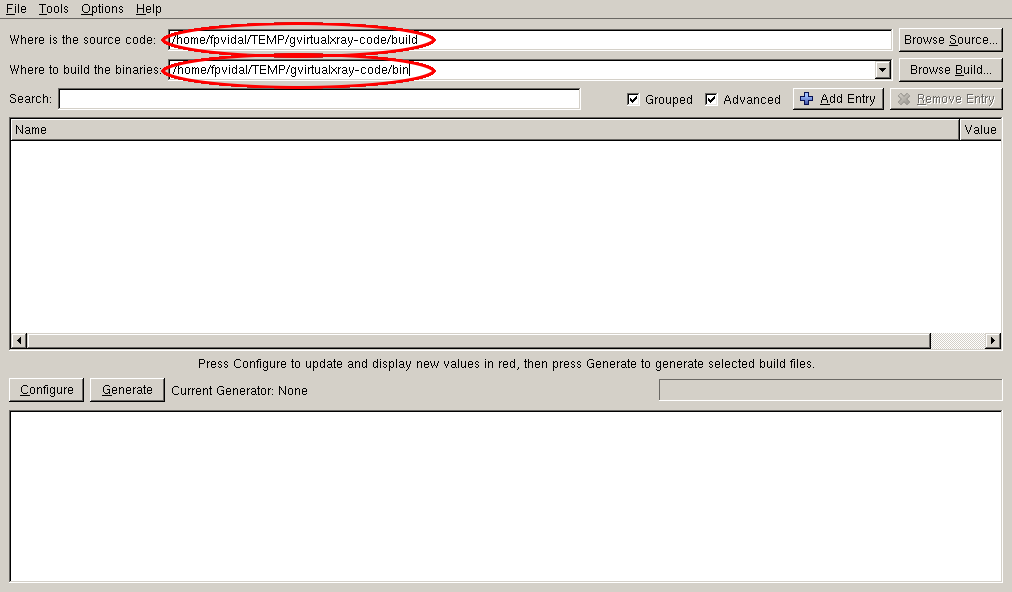
\includegraphics[width=0.5\linewidth]{cmake-01}\\
		\hline
		
		Click on \emph{Configure}:\\
		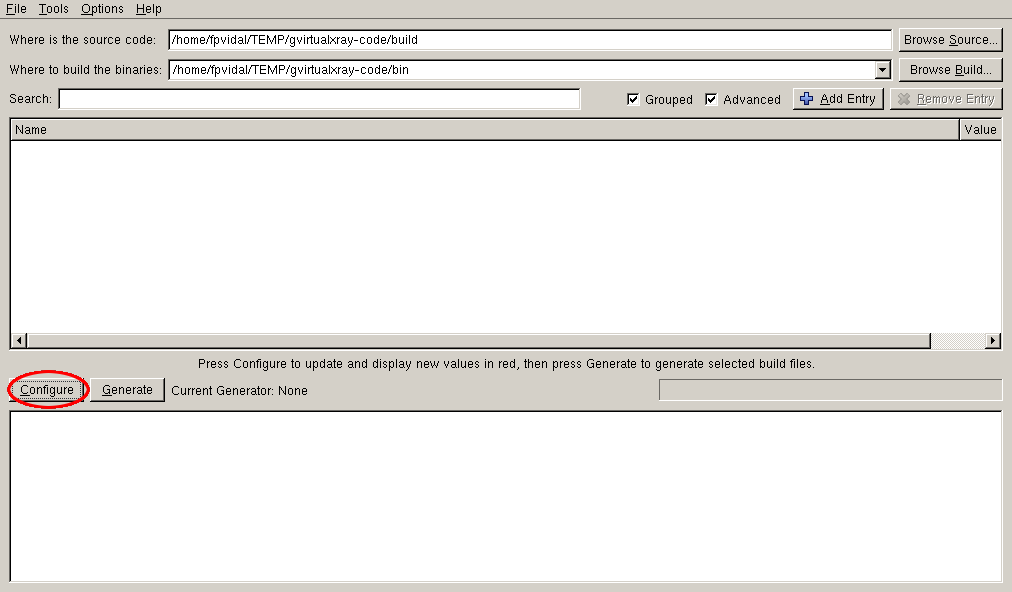
\includegraphics[width=0.5\linewidth]{cmake-02}\\
		\hline

		Select the generator that you wish to use:\\
		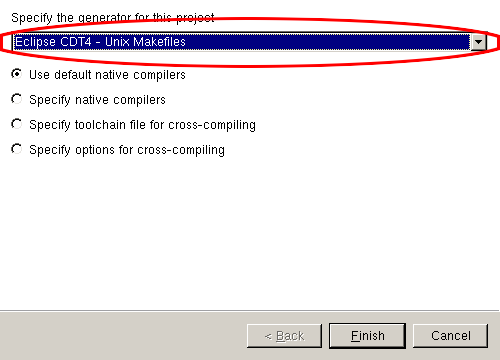
\includegraphics[width=0.35\linewidth]{cmake-03}\\
		\hline

		CMake will try to set up your development environment:\\
		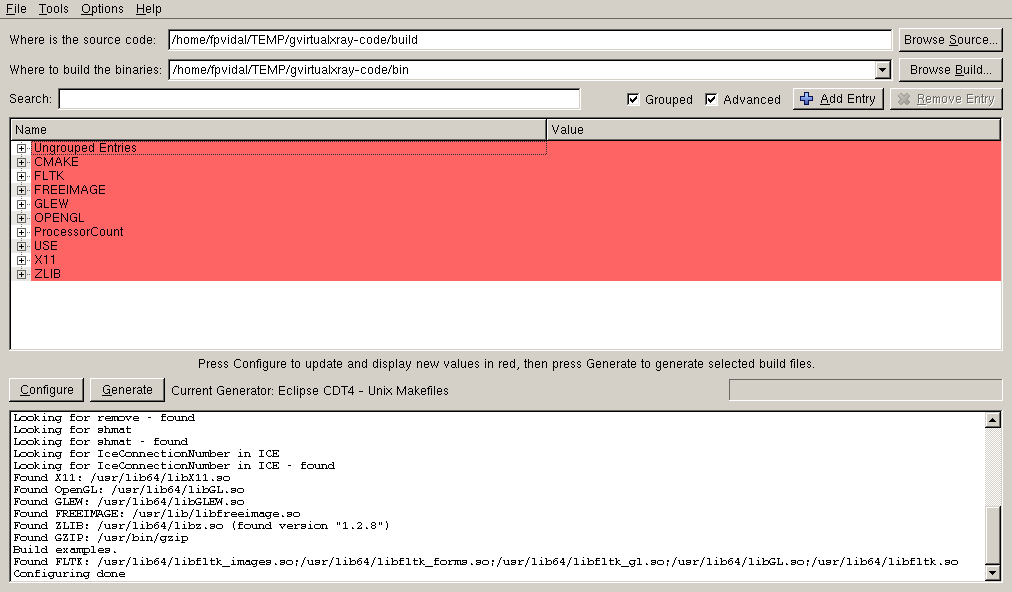
\includegraphics[width=0.5\linewidth]{cmake-04}\\
		\hline

		By default, the build type is Release, you can change it (with \emph{Debug}, \emph{MinSizeRel} or \emph{RelWithDebInfo}):\\
		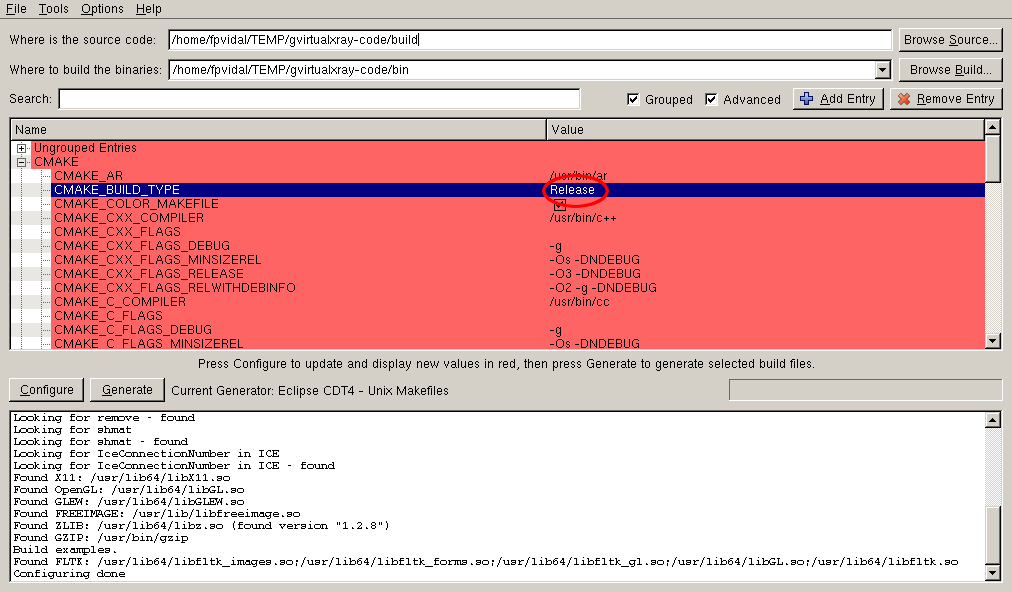
\includegraphics[width=0.5\linewidth]{cmake-05}\\
		\hline

		You can also manually modify or set the path to your libraries:\\
		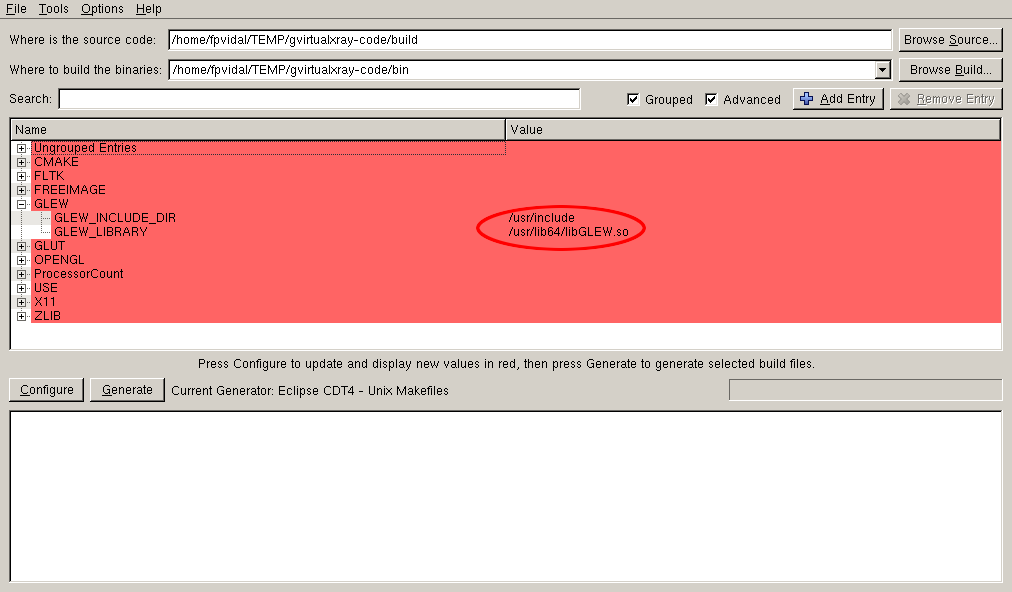
\includegraphics[width=0.5\linewidth]{cmake-09}\\
		\hline

		You can select different options, e.g. using \Gls{FLTK} or FreeGLUT (one or the other, not both), activate \Gls{ITK}:\\
		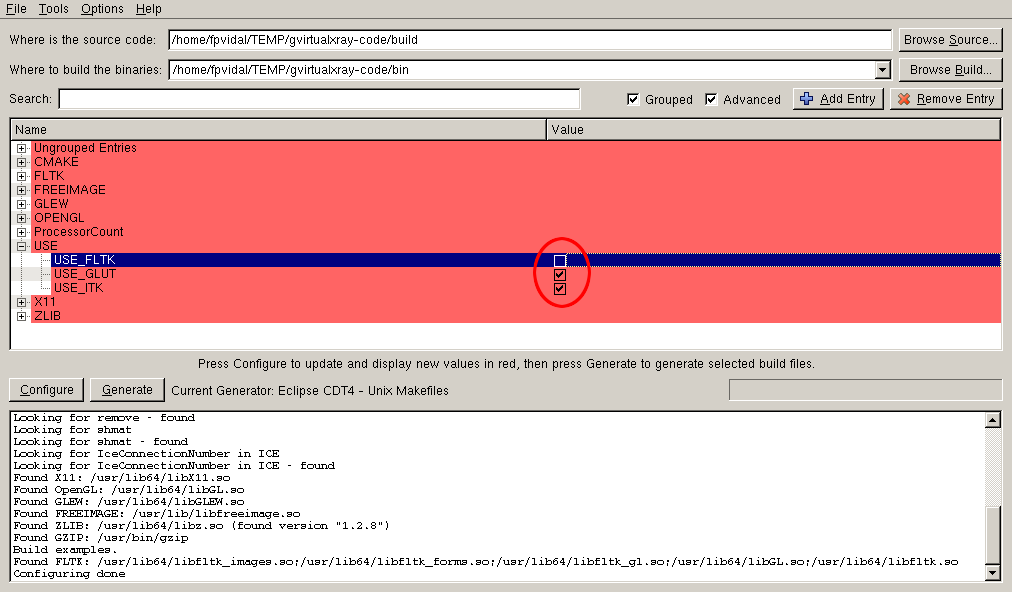
\includegraphics[width=0.5\linewidth]{cmake-06}\\
		\hline

		After any change, you have to press \emph{Configure} again so that the changes are effective:\\
		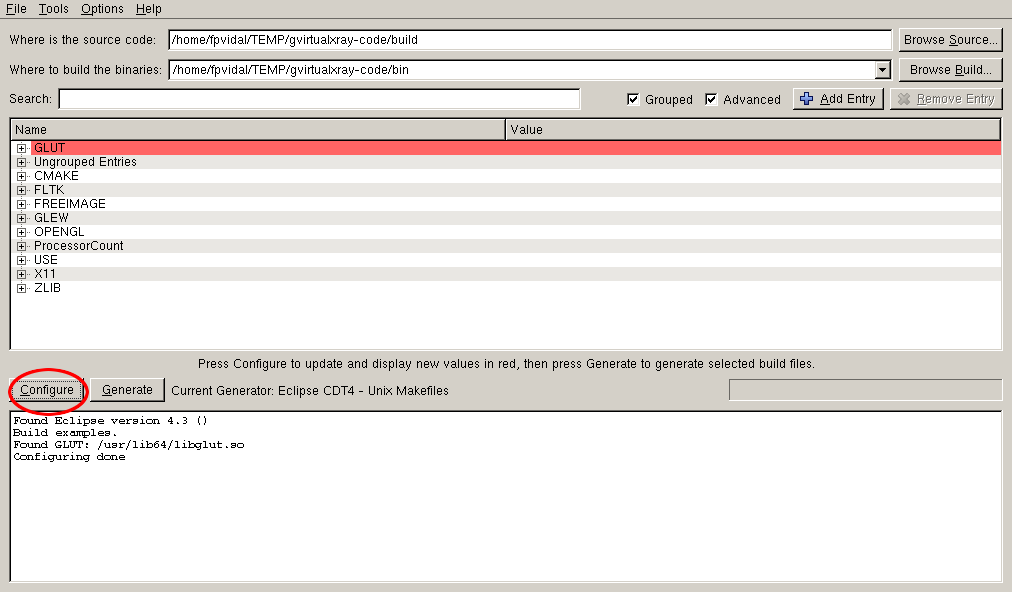
\includegraphics[width=0.5\linewidth]{cmake-07}\\
		\hline

		Once you have configured the project, click on \emph{Generate}.
		You are now ready to build the project with your selected development environment.\\
		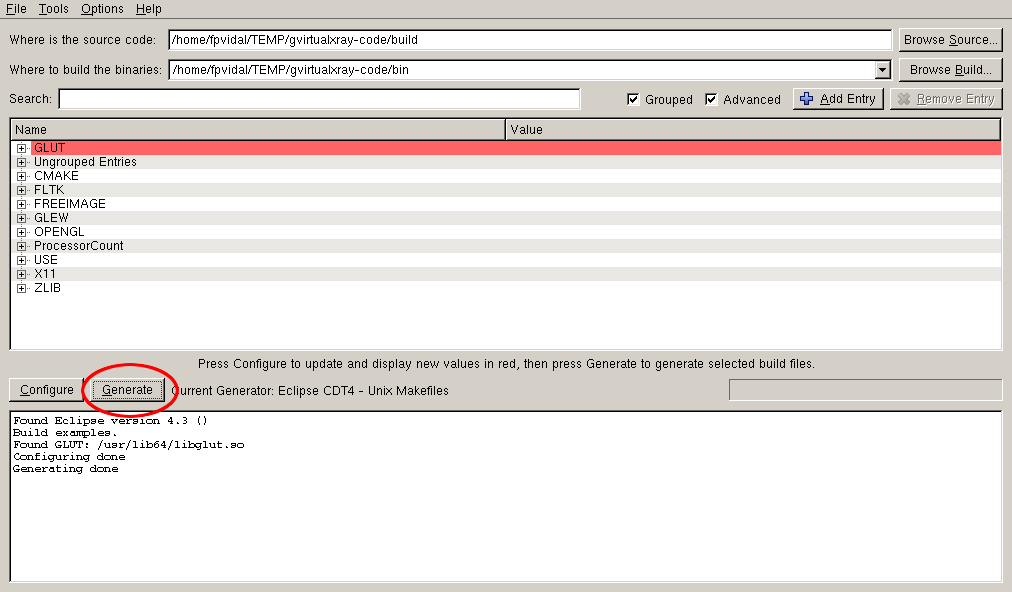
\includegraphics[width=0.5\linewidth]{cmake-08}\\
		\hline
	\end{longtable}
\end{center}

To make it a little easier on Windows platforms, it might be worth setting up environment variables to specify where you have installed some of the development tools/libraries. 
Here is a list of the variables that may be useful to set:

\begin{itemize}
	\item \Gls{Gzip}:
	\begin{itemize}
		\item \verb|GZIP_TOOL|
	\end{itemize}

	\item \Gls{GLEW}:
	\begin{itemize}
		\item \verb|GLEW_INCLUDE_DIR|
		\item \verb|GLEW_LIBRARY|
	\end{itemize}
	
	\item Zlib:
	\begin{itemize}
		\item \verb|ZLIB_INCLUDE_DIR|
		\item \verb|ZLIB_LIBRARY|
	\end{itemize}
	
	\item Boost:
	\begin{itemize}
		\item \verb|Boost_DIR|
	\end{itemize}

	\item If you use FreeGLUT:
	\begin{itemize}
		\item \verb|GLUT_INCLUDE_DIR|
		\item \verb|GLUT_LIBRARY|
	\end{itemize}

	\item Or if you use \Gls{FLTK}:
	\begin{itemize}
		\item \verb|FLTK_INCLUDE_DIR|
		\item \verb|FLTK_BASE_LIBRARY|
		\item \verb|FLTK_FLUID_EXECUTABLE|
		\item \verb|FLTK_FORMS_LIBRARY|
		\item \verb|FLTK_GL_LIBRARY|
		\item \verb|FLTK_IMAGES_LIBRARY|
		\item \verb|FLTK_MATH_LIBRARY|
	\end{itemize}

	\item If you use GLFW:
	\begin{itemize}
		\item \verb|glfw_DIR|
	\end{itemize}

	\item If you use \Gls{ITK}:
	\begin{itemize}
		\item \verb|ITK_DIR|
		\item And maybe \verb|VTK_DIR| if \Gls{ITK} was compiled with \Gls{VTK} support
	\end{itemize}
	
	\item If you use XCOM:
	\begin{itemize}
		\item \verb|XCOM_PATH|
	\end{itemize}

	\item If you use FreeType:
	\begin{itemize}
		\item \verb|FREETYPE_INCLUDE_DIR_freetype2|
		\item \verb|FREETYPE_INCLUDE_DIR_ft2build|
		\item \verb|FREETYPE_LIBRARY|
	\end{itemize}

% 	\item If you use FreeImage:
% 	\begin{itemize}
% 		\item \verb|FREEIMAGE_INCLUDE_DIR|
% 		\item \verb|FREEIMAGE_LIBRARY|
% 	\end{itemize}

\end{itemize}


\section{Tested platforms}

Successful compilation and installation have been tested on:

\begin{itemize}
 \item Linux openSUSE 12.3 (x86\_64) using the native compiler (g++ 4.7.2).
 \item Linux openSUSE 12.3 (x86\_64) using the Windows cross compiler (mingw32-g++ 4.8.1) provided by \Gls{MXE}.
 \item Linux openSUSE 13.2 (x86\_64) using the native compiler (g++ 4.8.3).
 \item Windows 8.1 (x86\_64) using Visual C++ 2010 in 32 bits.
 \item Windows 7 (x86) using Visual C++ 2013 in 32 bits.
 \item Mac OS X 10.8 (x86\_64) using the native compiler (LLVM 4.2) in 64 bits.
 \item Mac OS X 10.8 (x86\_64) using the GNU compiler (g++ 4.7) in 64 bits.
 \item Mac OS X 10.8 (x86\_64) using the Windows cross compiler (mingw32-g++ 4.8.1) provided by \Gls{MXE}.
\end{itemize}


\newpage
\printglossary[type=\acronymtype] 

\newpage
\phantomsection
\addcontentsline{toc}{section}{References}
\printbibliography


\end{document}
